\documentclass[12pt,aspectratio=169]{beamer}
\usetheme[version=2024]{iiasa}

\usepackage[
  maxnames = 1,
  style = authoryear,
  giveninits,
  terseinits,
  maxcitenames = 3,
  ]{biblatex}
\addbibresource{all.bib}

\usepackage{minted}
\setminted{
  fontsize=\footnotesize,
}
\renewcommand{\mod}[1]{\mintinline{python}{#1}}
\newcommand{\func}[1]{\mintinline{python}{#1()}}
\newcommand{\py}[1]{\mintinline{python}{#1}}

\setcounter{secnumdepth}{3}

\title{Model data pre- and post-processing with \texttt{genno}}

\date{
  \texorpdfstring{Message Community Meeting — Tuesday, 20 May 2025}%
  {2025-05-20}}

\author{\texorpdfstring{Paul Natsuo Kishimoto\\
  \href{mailto:kishimot@iiasa.ac.at}{\ttfamily \scriptsize <kishimot@iiasa.ac.at>}%
  }{Paul Natsuo Kishimoto <kishimot@iiasa.ac.at>}}

\begin{document}

\maketitle

\section{Whence and why \texttt{genno}?}

\subsection{Origin story, design goals, and outcomes}

\begin{frame}<1>[label=origin-story]
\frametitle{Origin story}

\structure{\bfseries ‘Reporting’} means to take the ‘raw’ model solution
and produce things of interest: derived data, tables, figures, etc.
\begin{itemize}
  \item In other words: \emph{everything} that happens after the GAMS/CPLEX optimizer
    finds optimal values for MESSAGE variables like \texttt{CAP}, \texttt{ACT}, etc.
\end{itemize}

\pause
\medskip
We have (and still use) some reporting code developed during a 2018 ‘hackathon’.
In 2019 we identified issues with this code, chiefly:

\begin{description}
  \item [Complexity] the code is on the order of 5000–10000 lines,
    bigger than the model ‘core’ and the code used to set up the model.
  \item [Performance] the code can take longer to run than the optimizer itself.
\end{description}

\medskip
We set out to address these issues.
\end{frame}

\begin{frame}[label=data-stages]
\frametitle{Workflow stages and data flows}

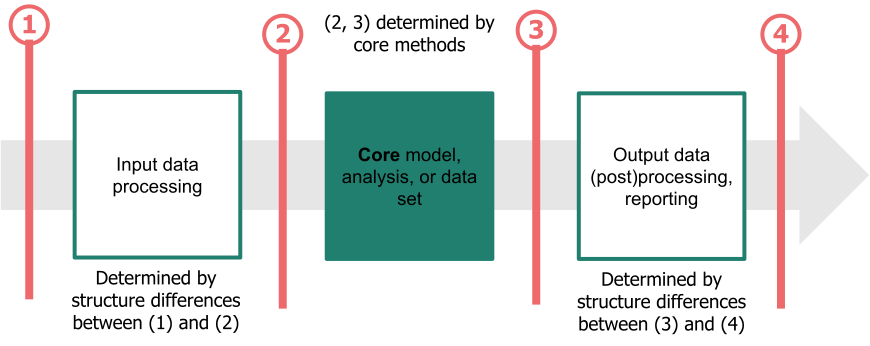
\includegraphics[width=\columnwidth]{data-stages}

\end{frame}

\againframe<2>{origin-story}

\begin{frame}
\frametitle{Outline}

\tableofcontents

\end{frame}

\begin{frame}[allowframebreaks]
\frametitle{Design goals}
We had many of these, but most importantly:

\bigskip
\structure{\bfseries Build on upstream packages} with high quality and performance.

\begin{description}
  \item [Performance] \mod{numpy}, \mod{pandas}, and others have good support for vectorized operations,
    and are regularly used for data \emph{much larger} than what goes in to/out of MESSAGE.
  \item [Quality] Many of these projects have full-time developers and maintainers.
    This makes them stable, relatively bug-free, well-documented, etc.
\end{description}

\medskip
Make \emph{full use} of their features instead of duplicating them.

\medskip
Provide only \emph{thin wrappers} and \emph{conveniences} that are easily maintained.

\framebreak
\structure{\bfseries Automate} repetitive tasks.

\begin{description}
  \item [High-level] common operations that one ‘nearly always' wants to do
    when working with MESSAGE data. (Examples to come.)
  \item [Low-level] handle dimensionality, sparsity of our data.
    Handle unit alignment, conversion, and derivation.
\end{description}

In both cases, make it easy to do the “right” (correct and performant) thing.
\emph{Reduce} cases where modelers have to duplicate or re-write the same operations →
fewer chances for fragile or slow code.

\medskip

\structure{\bfseries Reduce workload} for developers and maintainers%
—especially in iterative model-building workflows that lead to tweaking and revising methods:
\begin{itemize}
  \item Make complex methods more easily traceable.
\end{itemize}
\end{frame}

\begin{frame}
\frametitle{Design outcomes}
This led to a core set of capabilities that we packaged as \mod{genno}.

The name (“hammer” in Japanese) is a reference to the saying:

\begin{quote}
  “When you have a hammer, every problem looks like a nail.”
\end{quote}

…which can remind us of George Box's famous saying:
\begin{quote}
  “All models are wrong, but some are useful.”
\end{quote}

\begin{itemize}
  \item It turns out these affordances (features) are also very useful
    for \structure{pre-}processing: dealing with the data that go \emph{in} to the core model.
  \item Thus, for instance, the model-build process for MESSAGEix-Transport
    is structured as a set of genno operations.

    This has given us flexibility to make workflow changes required for many ongoing projects.
\end{itemize}
\end{frame}

\subsection{Basic concepts: chained operations vs. task graphs — quantities}

\begin{frame}[fragile]
\frametitle{Basic concepts: chained operations}
If you've used \mod{pandas},
you will have seen code like this:
(\href{https://github.com/iiasa/message-ix-models/blob/7a999bc0c636f0afea73f89f12e5cfe593d6d23c/message_ix_models/tools/iamc.py#L240-L254}
{from \mod{message_ix_models}})

\begin{columns}
\column{0.45\paperwidth}
\begin{minted}{python}
data.drop(columns=drop or [])
.query(query)
.replace(replace or {})
.dropna(how="all", axis=1)
.rename(columns=lambda c: c.upper())
.pipe(_raise_empty, query=query)
.pipe(_drop_unique, columns=unique, ...)
.pipe(_assign_n, missing=non_iso_3166)
.dropna(subset=["n"])
.drop("REGION", axis=1)
.set_index(set_index)
.rename(columns=lambda y: int(y))
.rename_axis(columns="y")
.stack()
.dropna()
\end{minted}

\column{0.45\paperwidth}
\pause
This pattern is called \structure{\bfseries chained operations}:
\begin{itemize}
  \item Each method call (like \py{.rename()}) \emph{acts on}
    the data structure: usually a \py{pandas.DataFrame} from the previous step.
  \item Each call \emph{returns} a modified frame that is input to the next step/operation, etc.
\end{itemize}

This code \emph{can be} compact and performant.
\end{columns}
\end{frame}

\begin{frame}
\frametitle{Challenges and pitfalls in using plain \texttt{pandas}}

Some issues we noted with our ‘legacy' reporting code:

\bigskip
\begin{itemize}
  \item Using \mod{pandas} chaining effectively takes \structure{careful coding}.

    It's (too) easy to fall back to e.g. nested loops → very slow code.
  \item It's not simple to:
    \begin{itemize}
      \item \structure{reuse an intermediate product} from a chain%
        —branch and carry on 2+ further chains without having to recompute.
      \item \structure{trace and step-through} intermediate steps in a long chain.
    \end{itemize}
  \item It's challenging to deal with \structure{operations involving multi-dimensional quantities}.

    For MESSAGE, we have to handle e.g. the
    \texttt{input} parameter (10-D),
    \texttt{ACT} variable (6-D), etc.
\end{itemize}
\end{frame}

\begin{frame}
\frametitle{Basic concepts: task graphs (\texttt{dask})}
The core logic of \mod{genno} relies on a package named \mod{dask}.

\medskip
Dask is built and used for truly \structure{‘Big’ Data}:
\begin{itemize}
  \item Imagine you have data spread across 10s or 100s of computers
    and want to do some operation on it—say, compute an average.
  \item Break this task into smaller tasks:
    \begin{enumerate}
      \item On each machine: load the local data,
        compute its average \emph{and} number of data points.
      \item Return these intermediate values to a 'master' machine/process.
      \item Aggregate the sub-averages to an overall average.
    \end{enumerate}
  \item Distribute these tasks across machines.
\end{itemize}
\end{frame}

\begin{frame}
\frametitle{Basic concepts: task graphs (\texttt{dask})}
\begin{columns}
\column{0.45\paperwidth}
In order to prepare and execute this kind of algorithm,
the atomic tasks can be viewed as a \structure{\bfseries graph}
of \structure{nodes} (tasks)
and \structure{edges} (data that's output from one task/input to the next).

\medskip
\onslide<2>{
This nodes-and-edges paradigm is also useful on a single machine.

\medskip
\mod{genno} uses \mod{dask}'s performant features for executing graphs of calculations.
\mod{genno} adds many conveniences to make it easy to assemble these graphs.
}

\column{0.45\paperwidth}
\includegraphics[width=\columnwidth]{Directed_acyclic_graph_2.pdf}
\end{columns}
\end{frame}

\begin{frame}
\frametitle{Quantities (\texttt{xarray}, \texttt{pandas}, and \texttt{pint})}

\mod{xarray}: another high-quality package that provides data structures like \py{xr.DataArray}
for \structure{labeled N-dimensional data}.
\begin{itemize}
  \item Example: climate data with dimensions (latitude, longitude, elevation, time)
    for multiple measures like temperature (°C) and pressure (kPa).
  \item Contrast with:
    \begin{itemize}
      \item \mod{numpy}: N-dimensional, but no text labels.
      \item \mod{pandas}: text labels, but first-class support only for 2-D (row, column) data.
    \end{itemize}
\end{itemize}

\medskip\pause
\mod{genno} provides a \py{Quantity} class that:
\begin{itemize}
  \item has the same interface as \py{xr.DataArray}.
  \item handles large, ‘sparse' data—using \mod{pandas} internally for performance.
  \item carries and handles units for entire quantities—using \mod{pint}.
\end{itemize}
\end{frame}


\begin{frame}[fragile,plain]

\begin{minted}{python-console}
>>> from genno import Quantity as Q
>>> days = {"day": ["Mon", "Tue"]}               # Dimension ID & labels
>>> q1 = Q([1.0, 2.0], units="km", coords=days)  # 1-D quantity
>>> q2 = Q(1.0, units="mile")                    # 0-D quantity
>>> q1 + q2                     # Alignment and compatible units handled
day
Mon    2.609344
Tue    3.609344
dtype: float64, units: kilometer

>>> q3 = Q([10., 8.], units="km/h", coords=days)
>>> q1 / q3                                       # Units are derived
day
Mon    0.10
Tue    0.25
dtype: float64, units: hour
\end{minted}

\end{frame}

\subsection{Operations and operators}

\begin{frame}
\frametitle{Operations and operators}

Following \mod{dask}, in \mod{genno} an ‘operator’ is \structure{any Python function or callable}.
\begin{itemize}
  \item May be simple (“Compute $f(x,y) = x^y$”) or complex (“Compute the logit share weight algorithm according to Kyle et al. (2010)”).
  \item Any number of inputs that can be N-dimensional quantities or other types.
  \item Can output Quantity or anything else.
\end{itemize}

\medskip
A growing library → pick-and-reuse instead of writing new code:
\begin{description}
  \item [\ttfamily genno] 42 operators%
    —basic arithmetic,
    manipulate dimensions, labels, and units,
    compatibility with SDMX and IAMC data structures.
  \item [\ttfamily ixmp] 7 operators%
    —retrieve/store Scenarios, time-series–, and model data
  \item [\ttfamily message\_ix] 4 operators%
    —construct and handle data for MESSAGE parameters.
  \item [\ttfamily message-ix-models] 20 general operators; 53 incl. MESSAGEix-Transport.
\end{description}
\end{frame}

\section{Reporting / post-processing}

\begin{frame}[allowframebreaks]
\frametitle{Reporting: some example requirements}
Some selections from a long list collected in 2019:

\medskip
We want to \structure{\bfseries compute the product} of:
\begin{itemize}
  \item \texttt{input}: a MESSAGE parameter with 10 dimensions
    that we can write as \texttt{nl-t-yv-ya-m-no-c-l-h-ho}.
  \item \texttt{ACT:nl-t-yv-ya-m-h}: a 6-D (solution) variable,

    dimensions overlap with \texttt{input}.
\end{itemize}

\medskip
Call this product \texttt{input:* × ACT:* =} \texttt{in:nl-t-yv-ya-m-no-c-l-h-ho}.
\begin{itemize}
  \item For some calculations, we'll want to use \emph{all the dimensions}.
  \item For others, we want to sum/average over \emph{different subsets} of them.
\end{itemize}

\framebreak
Often, reported data is destined for an instance of the IIASA Scenario Explorer
(like the IPCC AR6 SE, Scenario Compass, etc.).
This means it has to be \structure{\bfseries trasformed to the IAMC data structure}.
\begin{itemize}
  \item This has 6–7 dimensions:

    \texttt{model-scenario-region-variable-unit-year}.
  \item \texttt{model}, \texttt{scenario} are fixed for a given MESSAGEix Scenario.
  \item We want to specify that:
    \begin{itemize}
      \item \texttt{region} dimension labels are constructed from \texttt{nl} and/or \texttt{no}.
      \item \texttt{variable}: from some combination of \texttt{t-m-c-l},

        prefixed by a name for \emph{what} is being measured.

        e.g. \py{"Energy Service|Transportation|Passenger|2-wheelers"}
      \item \texttt{unit}: consistent with any intermediate operations.
    \end{itemize}
\end{itemize}


\framebreak
We want to do \structure{many, similar} such transformations
and then \structure{concatenate} them together.

\bigskip
We want to both \structure{write to file}
\emph{and} \structure{store in an ixmp database} these IAMC-structured data.

\bigskip
We want to also \structure{produce \emph{other} output files or data},
tailored to specific models/tools/code.

\end{frame}

\subsection{Example: ‘collecting' multiple outputs}

\begin{frame}[allowframebreaks,fragile]
\frametitle{Simple example: ‘collecting' multiple outputs}

\begin{columns}[T]
\column{0.45\textwidth}
\begin{minted}{python-console}
>>> def speak(sound: str):
...     print(f"{sound.title()}!")
>>> speak("hi")
Hi!

>>> from genno import Computer
>>> c = Computer()
>>> c.add("cow", speak, "moo")
>>> c.add("pig", speak, "oink")
>>> c.add("both", ["cow", "pig"])
>>> c.get("both")
Oink!
Moo!
\end{minted}

\column{0.45\textwidth}
\begin{minted}{python-console}
>>> c.add("hen", speak, "cluck")
>>> c.add("all three", ["both", "hen"])
>>> c.get("all three")
Oink!
Moo!
Cluck!

>>> c.visualize("example.svg",
...    "all three", rankdir="LR")
\end{minted}

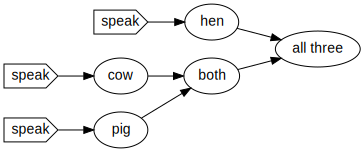
\includegraphics[width=\columnwidth]{genno-example.pdf}
\end{columns}

\framebreak
\begin{columns}[T]
\column{0.4\paperwidth}
\begin{minted}{python-console}
>>> print(c.describe("all three"))
'all three':
- list of:
  - 'both':
    - list of:
      - 'cow':
        - <function speak>
        - moo
      - 'pig':
        - '<function speak>' (above)
        - oink
  - 'hen':
    - '<function speak>' (above)
    - cluck
\end{minted}

\column{0.5\paperwidth}
Just as simple to have \emph{dozens} of such effects, calculations, and output files.

\smallskip
One key \py{"transport all"} for MESSAGEix-Transport produces:
\begin{itemize}
  \item ‘Main' IAMC-structured output to CSV and Excel.
  \item 16 PDF documents with multiple pages of plots.
  \item 24 files with intermediate quantities for debugging.
  \item 5 SDMX data flows + structural metadata for some collaborators.
\end{itemize}
\end{columns}
\end{frame}

\begin{frame}
\frametitle{Full task graph to report \texttt{"transport all"}}

\hspace*{-10mm}
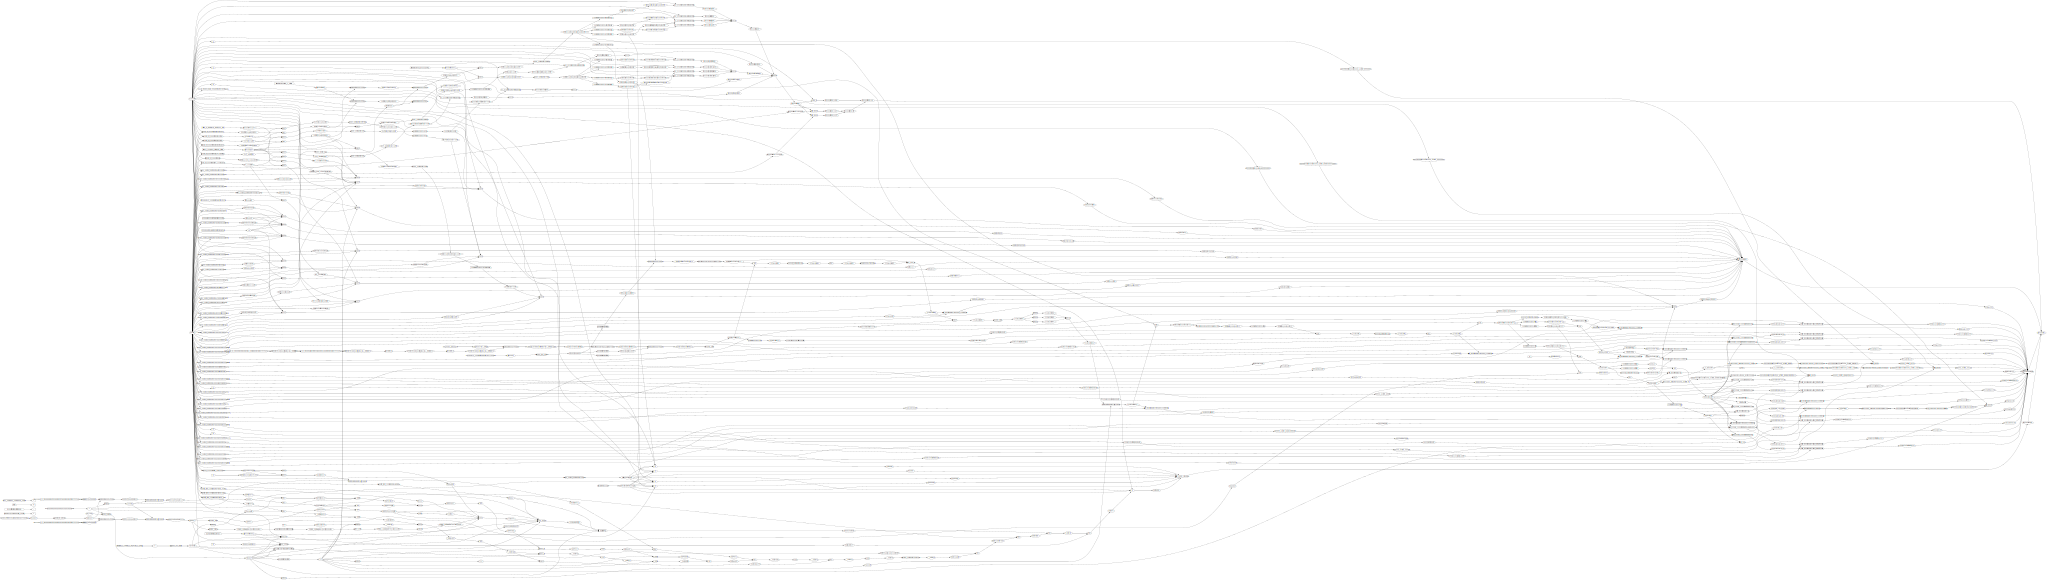
\includegraphics[width=\paperwidth]{transport-report.pdf}

\end{frame}

\begin{frame}[plain]

\vspace*{-1mm}
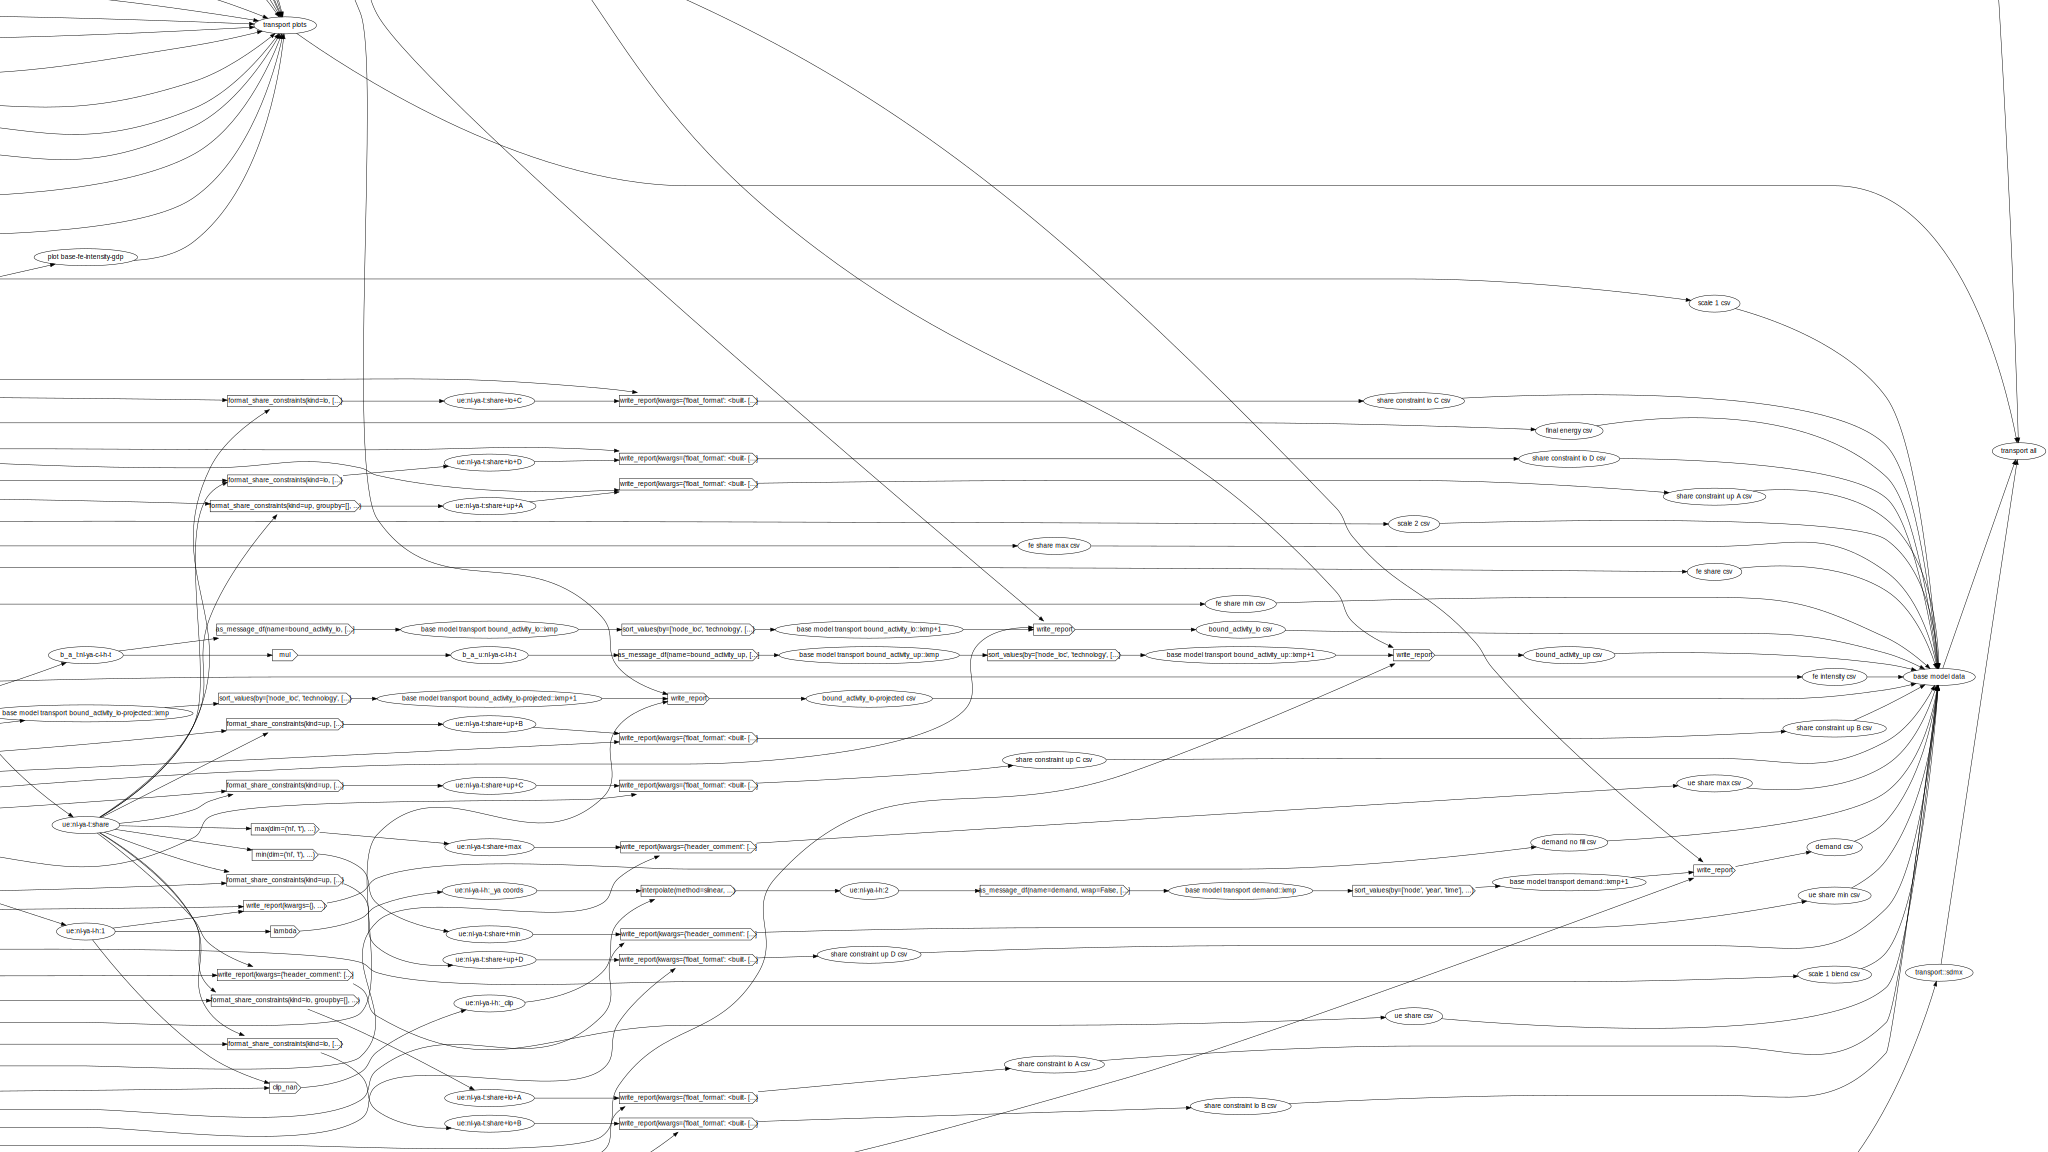
\includegraphics[height=0.9\textheight]{transport-report-crop.pdf}

\end{frame}

\subsection{Features for developing reporting}

\begin{frame}
\frametitle{Features for developing reporting}
\vspace*{-2mm}
Reporting is developed iteratively as part of the model-building process.

Besides the describe/visualize features,
\mod{genno} can be used in this process to:

\begin{columns}[T]
\column{0.45\paperwidth}
Mix automatic \& custom tasks.
\begin{itemize}
  \item \mod{message_ix} creates a graph with ca. 16,000 possible tasks (\texttt{dask} skips unused ones).
  \item We can add, remove, or replace these using further code.

    e.g. \mod{message_ix_models} adds tasks for modules (transport, buildings, etc.) or projects.
\end{itemize}

Compute intermediate values to debug.

\column{0.45\paperwidth}
Integrate with tests via in-line or ‘pass-through' checks.
\begin{itemize}
  \item Make assertions about the Quantity/data produced
    at a certain point in the graph—then carry on.
  \item e.g. data is produced for expected numbers/lists of nodes or techs.
  \item e.g. data have certain units or dimensionality.
\end{itemize}
\end{columns}
\end{frame}

\section{Model data prep / pre-processing}

\againframe{data-stages}

\begin{frame}
\frametitle{Model data preparation}

In some ways, this is the dual or mirror-image of reporting:

\structure{\bfseries FROM} a variety of input data sources:
\begin{itemize}
  \item Files from many data providers, in varied formats, structure, resolution.
  \item Partial-coverage requiring assumptions to fill, broadcast, extrapolate, etc.
  \item Configurable (scenario-specific) assumptions.
  \item Existing data in a Scenario, to be modified
\end{itemize}

\medskip
\structure{\bfseries TO} the specific structure of MESSAGE parameters
(\texttt{input}, \texttt{output}, \texttt{inv\_cost}, \texttt{growth\_new\_capacity\_up}, etc.).
\begin{itemize}
  \item Data must be complete: all dimensions populated, even if not used.
  \item Data must be consistent, else model will not be feasible/accurate.
\end{itemize}

\smallskip
Just like reporting, these many operations can be neatly organized using \mod{genno}.
\end{frame}

\begin{frame}
\frametitle{Full task graph to build \texttt{"add transport data"}}

\hspace*{-10mm}
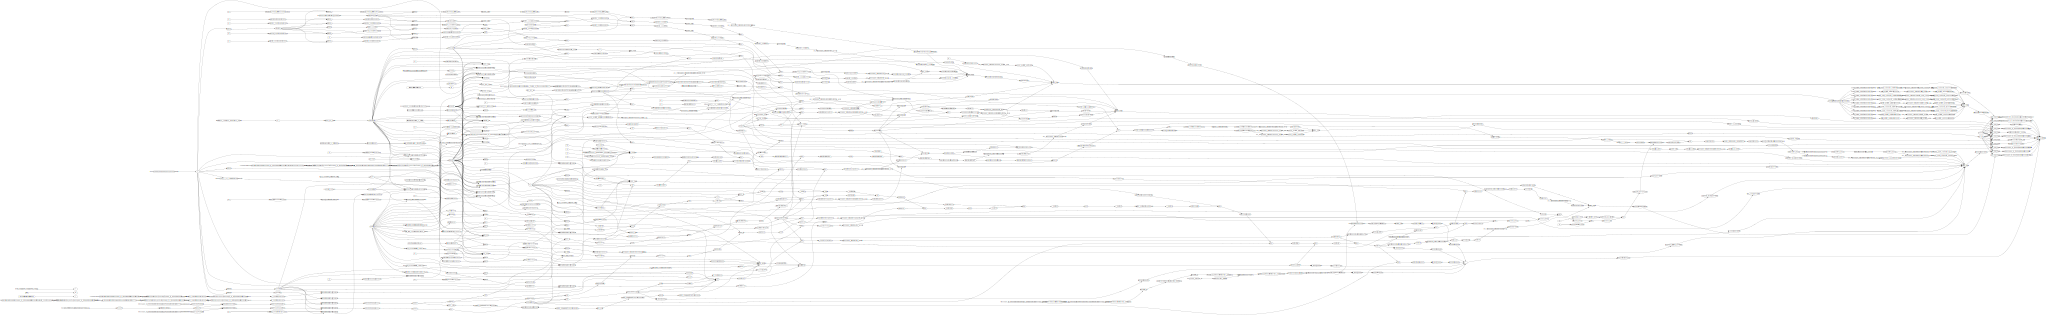
\includegraphics[width=\paperwidth]{transport-build.pdf}

\end{frame}

\begin{frame}[plain]

\vspace*{-1mm}
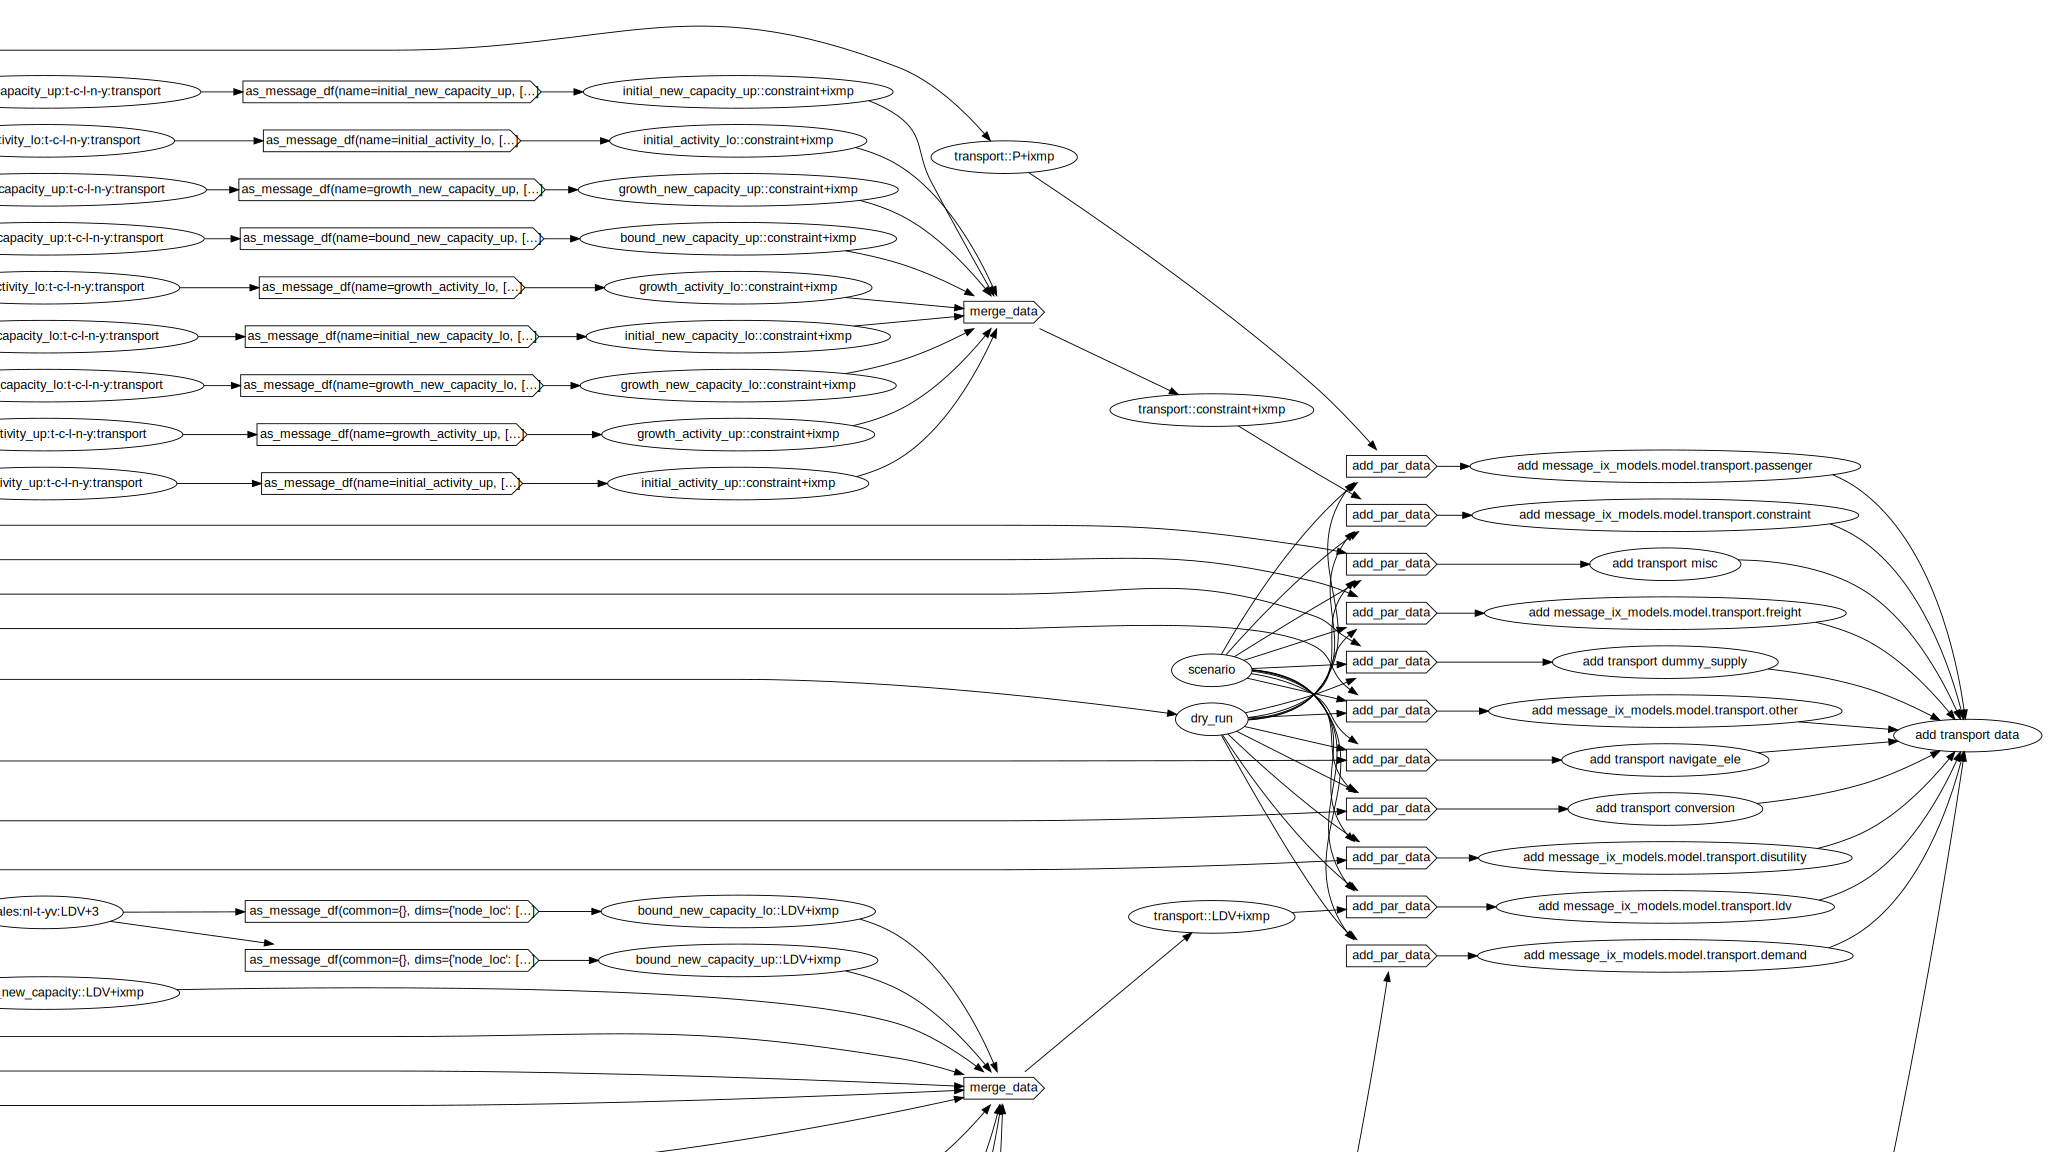
\includegraphics[height=0.9\textheight]{transport-build-crop.pdf}

\end{frame}

\subsection{Example: \texttt{demand} in MESSAGEix-Transport}

\begin{frame}
\frametitle{Example: MESSAGEix-Transport \texttt{demand}}

Parameter values for every \texttt{node-commodity-level-year-time}:
\begin{itemize}
  \item Measure: total passenger-distance travelled (PDT) in 10⁹ km / year.
  \item \texttt{commodity}: 5 modes, 2W AIR BUS LDV RAIL, e.g. \py{"transport passenger 2W"}
\end{itemize}

\medskip\pause
Our “standard" setup implements a specific method:
\begin{enumerate}
  \item GDP and population \structure{→ compute} GDP/capita.
  \item Base-year (t=0) PDT values and GDP \structure{→ project} future total PDT/capita.
  \item Other input data \structure{→ compute} a \texttt{mode share:n-t-y}.

     \only<2>{E.g. (n=R12\_SAS, y=2060, t=2W) = 0.2 → 20\% of all PDT is by the 2W mode.}
  \pause
  \item Product of (2) and (3) \structure{→} PDT/capita for each \texttt{n-t-y}.
  \item Product of (4) and population
    \structure{→} \texttt{total pdt:n-t-y}
    \structure{→} \texttt{demand:n-t-y}.
  \item \texttt{demand:n-t-y}, a genno Quantity \structure{→ convert} to MESSAGE data frame.
  \item (6) and target scenario \structure{→ add/update} the data.
\end{enumerate}
\end{frame}

\begin{frame}[allowframebreaks]
\frametitle{Modifying methods for project needs}

For certain projects, we imagine particular scenarios where behavioural changes, digitalization, and other phenomena change how LDVs are used.
\begin{itemize}
  \item Our partners in these projects produce \structure{new data files} with

    (a) total LDV \emph{vehicle}-distance travelled (VDT) and

    (b) \emph{occupancy} of LDVs, for many countries.
\end{itemize}

\medskip
Since the standard method is built with \mod{genno}, this change is straightforward:

we ‘graft' these onto our existing task graph.
\begin{enumerate}
  \item [8.] New tasks to read, manipulate, aggregate new input files

    \structure{→ compute} a new quantity, \texttt{LDV pdt total:n-t-y} (n=LDV only).
  \item [9.] \texttt{pdt total:n-t-y} (5 on prev. slide)

    \structure{→ select} values for n $\in$ (2W AIR BUS RAIL) only.
  \item [10.] (8) and (9) \structure{→ concatenate} to produce \texttt{demand:n-t-y}.
\end{enumerate}

\framebreak
Tasks to compute the input at (9) are \emph{already} set up.

The key at (10) is \emph{already} the input to (6).

\medskip
All the rest of our input data preparation \structure{needs no changes} and \structure{operates exactly as before}.
\begin{itemize}
  \item ‘Upstream’ data, e.g. scenario-specific population, GDP, mode shares flow into the newly-added tasks.
  \item Other ‘downstream’ tasks receive different values, but don't need any changes.

    e.g. LDV PDT → VDT → implied stock of vehicles in base period.
\end{itemize}

\medskip

\medskip
For other projects, we can make different changes to the same or other keys in the task graph.
These can also be \structure{precise} and \structure{narrowly targeted}.
\end{frame}

\section{Conclusion and discussion}

\begin{frame}
\frametitle{Recap}

Specific needs of MESSAGE reporting and model-building

→ performance, stability, ease-of-use requirements

→ code to bring together existing, high-quality packages and meet those needs

→ \structure{\ttfamily genno}

\bigskip
Benefits:
\begin{itemize}
  \item Traceable, transparent.
  \item Simple code for even large task graphs with many steps.
  \item As performant as possible, without special effort.
  \item Reduce waste: duplication and consequent poor performance.
  \item Flexible, adaptable, reusable —both entire graphs and individual operators.
\end{itemize}

\end{frame}

\subsection{Learn more \& get involved}

\begin{frame}
\frametitle{Learn more \& get involved}

\begin{itemize}
  \item \href{https://docs.messageix.org/en/latest/tutorials.html\#westeros-electrified}{\mod{message_ix} reporting tutorial} (number 3.1)
    gives a full overview of the concepts and usage.
    Used in the regular MESSAGE Training Workshop.
  \item \href{https://genno.readthedocs.io/en/latest/}{\mod{genno} documentation} —complete and up to date.
  \item \href{https://docs.messageix.org/projects/models/en/latest/api/report/index.html}{\mod{message_ix_models.report}}
    —applied to reporting the MESSAGEix-GLOBIOM global model.
  \item \href{https://github.com/iiasa/message-ix-models/blob/main/message_ix_models/model/transport/ldv.py}{Code for \mod{message_ix_models.model.transport.ldv}}
    and other models that implement transport model data prep step-by-step, with explanatory comments.
  \item \href{https://github.com/iiasa/message_ix/discussions}{Discussions} on the \mod{message_ix} GitHub repository.
  \item …or reach out by e-mail or any other means!
\end{itemize}
\end{frame}

\makefinalslide

\end{document}
